\documentclass[a4paper,8pt]{article}

\usepackage[T1]{fontenc}
\usepackage[swedish]{babel}
\usepackage[utf8]{inputenc}

\usepackage{lmodern}
\usepackage{amsmath}
\usepackage{graphicx}
\usepackage{amsfonts}

% Tikz
\usepackage{tikz}
\usetikzlibrary{shapes,arrows}
\tikzstyle{block} = [rectangle, draw, 
    text width=5em, text centered, rounded corners, minimum height=4em]
\tikzstyle{line} = [draw, -latex']


\usepackage{bytefield}
\title{\huge{$\mu$8} \vspace{1cm}\\ 
  \large{TSEA43 - Kravspec}}
\author{Johan Angelstam, Caj Larsson, Erik Lindholm}
\date{2011-07-18}

\begin{document}

\maketitle
\vfill
\begin{tabular}{ l l l }
  Version & Datum & \\
  1.0     & 2011-07-18 & Första versionen \\
\end{tabular}

\thispagestyle{empty}

\pagebreak

\section{Beskrivning}
Vi vill bygga en mycket enkel 8-bitars dator med 2-bitars
opkod. Den styr någon typ av utmatningsenhet exempelvis en
D/A-omvandlare som då kan producera ljud och eventuellt något
musikliknande.

\section{Blockschema}
\begin{figure}[h]
\centering
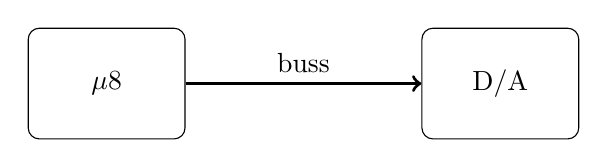
\begin{tikzpicture}[node distance = 5 cm, auto]
  \node [block] (MY8) {$\mu$8};
  \node [block, right of = MY8] (DA) {D/A};
  \draw [->, very thick] (MY8) to node {buss} (DA);
\end{tikzpicture}
\end{figure}

\section{Krav}
För att inte sätta ribban för högt har vi varit tämligen restriktiva med våra
 ska-krav.

\subsection{Ska}
\begin{enumerate}
  \item CPU med 8-bitars minnesbredd och 2-bitars opkod.
  \item Opkod för utmatning via 8-bitarsbussen.
\end{enumerate}

\subsection{Bör}
\begin{enumerate}
  \item 
\end{enumerate}

\end{document}
